\documentclass[conference]{IEEEtran}

\usepackage{cite}
\usepackage{amsmath,amssymb,amsfonts}
\usepackage{mathrsfs}
\usepackage{bm}
\usepackage{graphicx}
\usepackage{epstopdf}
\usepackage{tikz}
\usepackage{float}
\usetikzlibrary{positioning}


\newtheorem{theorem}{Theorem}
\newtheorem{lemma}{Lemma}
\newtheorem{remark}{Remark}
\newtheorem{asum}{Assumption}

\setlength{\textfloatsep}{0pt plus 2pt minus 2pt}
\setlength{\floatsep}{-4pt plus 1pt minus 1pt}
\setlength{\abovecaptionskip}{-6pt}
\setlength{\belowcaptionskip}{-4pt}


\begin{document}
	
	\title{Consensus Control for Multi-Agent Systems under Switching Topologies via State-Dependent Dwell-Time Switching}
	
	\author{
		\IEEEauthorblockN{1\textsuperscript{st} Yiming Wang}
		\IEEEauthorblockA{\textit{School of Mathematics}\\
			\textit{Liaoning Technical University}\\
			Fuxin, China\\
			wym2392940747@163.com}
		\and
		
		\IEEEauthorblockN{2\textsuperscript{nd} Jianxiang Ren}
		\IEEEauthorblockA{\textit{School of Mathematics}\\
			\textit{Southeast University}\\
			Nanjing, China\\
			jxren@seu.edu.cn}
		
		\and
		\IEEEauthorblockN{3\textsuperscript{rd} Xiao Fang}
		\IEEEauthorblockA{\textit{School of Automation}\\
			\textit{Southeast University}\\
			Nanjing, China\\
			fangxiao@seu.edu.cn}

\and
		\IEEEauthorblockN{4\textsuperscript{th} Dan Zhao}
		\IEEEauthorblockA{\textit{School of Automation}\\
			\textit{Southeast University}\\
			Nanjing, China\\
			danzhao@seu.edu.cn}}
	
	\maketitle
	
	\begin{abstract}
		This paper investigates the consensus problem for switched multi-agent systems with multiple candidate directed communication topologies. A consensus-orthogonal decomposition is first introduced to eliminate the redundant consensus component and transform the original multi-agent system into a reduced-order switched disagreement system. A state-dependent dwell-time switching law is then designed via Lyapunov-Metzler inequalities to stabilize the disagreement error system. Under the jointly strongly connected topology condition, the Lyapunov-Metzler inequalities are proved to be feasible for every prescribed minimum dwell time below an explicitly derived positive upper bound. It is shown that, the disagreement error converges to zero and global consensus is achieved, provided that the union of the candidate communication graphs is strongly connected. A numerical example is provided to illustrate the effectiveness of the proposed approach.
	\end{abstract}
	
	\begin{IEEEkeywords}
		Multi-agent consensus, switching topology, joint strong connectivity, Lyapunov-Metzler inequality, state-dependent dwell-time.
	\end{IEEEkeywords}
	
	\section{Introduction}
	
	Consensus control is a fundamental problem in multi-agent systems,
	where a group of agents is required to reach agreement through local
	information exchange over communication networks
	\cite{olfati2007,wen2021book}. Existing studies have extended consensus control
	to second-order systems with velocity and input constraints and
	finite-time protocols with actuator saturation
	\cite{fu2019constraints,zhao2015finite}. And resilient consensus for higher order multi-agent networks has also been investigated in \cite{zhao2019tracking}.

	
	In graph-based consensus analysis, connectivity of the communication
	topology plays a fundamental role. For undirected networks,
	connectivity is a standard condition for consensus
	\cite{olfati2004}, whereas directed networks are typically required
	to be strongly connected or to contain a directed spanning tree
	\cite{jadbabaie2003,ren2005}. In practical networked systems,
	however, communication topologies may switch due to link failures,
	sensing limitations, communication constraints, or intermittent
	information exchange. Representative studies have investigated consensus tracking of multi-agent systems with Lipschitz-type node dynamics under switching topologies \cite{wen2014tracking} and developed multiple-Lyapunov-function approaches to tracking control of multi-agent systems with switching topologies \cite{wen2019multiple}. Although a single candidate topology
	may be disconnected and fail to guarantee global consensus
	independently, the union of several candidate topologies may be
	strongly connected and provide sufficient information paths.
	Existing studies have shown that consensus can still be achieved
	under jointly connected switching topologies even when each
	individual topology is insufficient
	\cite{cheng2019,li2023}.
	
	An effective approach to consensus analysis is to separate the
	consensus and disagreement components. Through an orthogonal
	transformation, the original consensus problem can be converted into
	the stability problem of a reduced-order disagreement system
	\cite{wang2024protocol}. The resulting model removes the redundant
	consensus direction and permits the direct application of
	switched-system stability methods.
	
	The reduced disagreement dynamics constitute a switched system whose
	individual subsystem matrices may be unstable or marginally stable.
	Classical switched-system theory has shown that a suitable switching
	law can stabilize the overall system without requiring every
	subsystem to be Hurwitz
	\cite{liberzon2003,geromel2006,zhai2001}. More recent studies have
	developed mode-dependent dwell-time and multiple-Lyapunov-function
	methods for switched systems containing unstable modes
	\cite{jin2023,yin2023}. These results motivate treating consensus
	under individually disconnected topologies as a switched-system
	stabilization problem.
	
	This paper addresses the consensus problem in multi-agent systems with multiple
	candidate directed communication topologies. Each candidate topology
	is disconnected, whereas the union of all candidate topologies is
	strongly connected. Motivated by the state-dependent dwell-time
	framework in~\cite{russo2025}, a Lyapunov-Metzler-based switching
	mechanism is applied to the reduced-order disagreement dynamics. An
	orthogonal decomposition removes the consensus direction, and the
	proposed switching law drives the disagreement state to zero, thereby
	achieving global consensus.
	
	The main contributions are summarized as follows:
	\begin{itemize}
		\item A consensus-orthogonal decomposition is introduced to
		transform the original consensus problem into stabilization of a
		reduced-order switched disagreement system.
		
		\item A state-dependent switching law based on finite-dwell-time
		Lyapunov-Metzler inequalities is developed. The law enforces a
		prescribed minimum dwell time without requiring the individual
		subsystem matrices to be Hurwitz.
		
		\item A constructive feasibility analysis is established through
		a Hurwitz convex combination, a specially constructed Metzler
		matrix, and a lifted Lyapunov operator. An explicit sufficient
		upper bound on the prescribed dwell time is consequently derived.
	\end{itemize}
	
	The remainder of this paper is organized as follows. Section~II
	presents the graph preliminaries and reduced-order disagreement
	dynamics. Section~III introduces the state-dependent dwell-time
	switching law. Section~IV establishes the feasibility of the
	Lyapunov-Metzler inequalities. Section~V presents numerical
	simulations, and Section~VI concludes the paper.
	
	\emph{Notations:}
	$\mathbb R^n$ denotes the $n$-dimensional Euclidean space. The vector \(\mathbf 1_N\in\mathbb R^N\) stands for the $N$-dimensional all-ones vector. \(I_n\in\mathbb R^{n\times n}\) is the $n$-order identity matrix, and \(\mathbf 0_n\in\mathbb R^n\) denotes the $n$-dimensional zero vector. For a symmetric matrix $P$, $P\succ0$ and $P\prec0$ denote positive and negative definiteness. The symbol $\otimes$ denotes the Kronecker product. For square matrices $A$ and $B$, $A\oplus B=A\otimes I+I\otimes B$ denotes the Kronecker sum. For vectors, $\|\cdot\|_2$ is the Euclidean norm; for matrices, it is the induced spectral norm. For a square matrix $A$, $\operatorname{spec}(A)$ denotes its spectrum. The notation $\operatorname{col}\{\cdot\}$ denotes column stacking. For a matrix $X\in\mathbb R^{m\times n}$, $\operatorname{vec}(X)\in\mathbb R^{mn}$ denotes the column-wise
	vectorization obtained by stacking the columns of $X$. The class $\mathcal M$ contains Metzler matrices
	$\Pi=[\pi_{ij}]\in\mathbb R^{M\times M}$ satisfying
	$\pi_{ij}\geq0$ for $i\ne j$ and
	$\Pi\mathbf 1_M=\mathbf 0_M$. The set of real symmetric matrices of dimension $r$ is denoted by $\mathbb S^r$, and
	$\mathbb S_+^r=\{Z\in\mathbb S^r:Z\succeq0\}$ denotes the
	positive-semidefinite cone. The notation $(\mathbb S_+^r)^M$
	denotes its $M$-fold Cartesian product. For a matrix $Z$,
	$\ker(Z)$ denotes its null space. For a closed convex set
	$\mathcal K$ and $Z\in\mathcal K$, $T_{\mathcal K}(Z)$ denotes
	the tangent cone to $\mathcal K$ at $Z$.
	
	\section{Preliminaries and Problem Formulation}
	
	Consider $N$ agents with states $x_i(t)\in\mathbb R^d$,
	$i\in\mathcal V$, where
	$\mathcal V=\{1,\ldots,N\}$ is the agent set. Define
	$
	x(t)
	=
	\operatorname{col}\{x_1(t),\ldots,x_N(t)\}
	\in\mathbb R^{Nd}.
	$
	The communication network of these $N$ agents switches among $M$ candidate directed
	graphs
	$
	\mathcal G_p=(\mathcal V,\mathcal E_p),
	p\in\Omega=\{1,\ldots,M\},
	$
	where $\mathcal E_p\subseteq\mathcal V\times\mathcal V$ is the
	directed edge set. Define
	$\mathcal A_p=[a_{ij}^p]\in\mathbb R^{N\times N}$ as the weighted
	adjacency matrix. A directed edge $(j,i)\in\mathcal E_p$ means that
	agent $i$ can receive information from agent $j$. Accordingly, $a_{ij}^p>0$ if $(j,i)\in\mathcal E_p$, while $a_{ij}^p=0$ indicates the absence of the directed edge from agent $j$ to agent $i$. The associated Laplacian matrix \(L_p=[l_{ij}^p]\) satisfies
	$l_{ii}^p=\sum_{j\ne i}a_{ij}^p$, $l_{ij}^p=-a_{ij}^p$, $i\ne j,$
	which yields
	$L_p\mathbf1_N=\mathbf0_N$, $p=1,\ldots,M.$
	A directed path from agent $i$ to agent $j$ refers to a sequence of directed edges connecting agents $i$ to $j$. A directed graph is strongly connected if any agent is reachable from all other agents via a directed path. A family of directed graphs
	$\{\mathcal G_p\}_{p=1}^{M}$ is said to be jointly strongly
	connected if their union graph
	$
	\mathcal G_U
	=
	\bigcup_{p=1}^{M}\mathcal G_p
	$
	is strongly connected.
	
	\begin{asum}\label{ass:joint}
		Each candidate directed topology $\mathcal G_p$ is disconnected, whereas the family
		$\{\mathcal G_p\}_{p=1}^{M}$ is jointly strongly connected.
	\end{asum}
	
	Under the active topology $\mathcal G_{\sigma(t)}$, where
	$\sigma(t)\in\Omega=\{1,\ldots,M\}$ is the switching signal, the agent dynamics under the standard consensus protocol are
	given by
	\vspace{-0.2\baselineskip}
	\begin{equation}
		\dot{x}_i(t)
		=
		-\sum_{j=1}^{N}
		a_{ij}^{\sigma(t)}
		\bigl(x_i(t)-x_j(t)\bigr).
		\label{eq:agent_dynamics}
		\vspace{-0.2\baselineskip}		
	\end{equation}
	
	By stacking
	$
	x(t)=\operatorname{col}\{x_1(t),\ldots,x_N(t)\},
	$
	then \eqref{eq:agent_dynamics} can be written in compact form as
	\vspace{-0.2\baselineskip}
	\begin{equation}
		\dot{x}(t)
		=
		-\bigl(L_{\sigma(t)}\otimes I_d\bigr)x(t),
		\label{eq:original_system}		
		\vspace{-0.2\baselineskip}
	\end{equation}
	where $I_d$ is the $d$-dimensional identity matrix.
	
	The multi-agent system achieves consensus if
	$
	\lim_{t\to\infty}
	\bigl(x_i(t)-x_j(t)\bigr)
	=
	\mathbf 0_d
	$ for all $ i,j\in\{1,2,\ldots,N\},$ or equivalently when $x(t)$ converges to the consensus subspace $\mathcal{S}_c=\{\mathbf{1}_N\otimes\eta:\eta\in\mathbb{R}^d\}$.
	
	To describe the disagreement among agents, define the centering
	matrix
	$
	H
	=
	I_N-\frac{1}{N}\mathbf 1_N\mathbf 1_N^\top.
	$
	Let $S\in\mathbb R^{(N-1)\times N}$ satisfy
	$
	S\mathbf 1_N=\mathbf 0_{N-1},
	$
	$
	SS^\top=I_{N-1},
	$
	$
	S^\top S=H.
	\label{eq:S_properties}
	$
	Consequently, the rows of $S$ form an orthonormal basis of the subspace
	orthogonal to the consensus direction $\mathbf 1_N$.
	
	Define the reduced-order disagreement vector
	$
	\xi(t)
	=
	(S\otimes I_d)x(t)
	\in\mathbb R^r,
	$
	$
	r=(N-1)d.
	\label{eq:xi_definition}
	$
	Since $\operatorname{rank}(S)=N-1$ and $S \mathbf1_N=\mathbf 0_{N-1}$, we have
	$
	\ker(S)
	=
	\operatorname{span}\{\mathbf 1_N\},
	$
	which implies that \(\xi(t)=\mathbf 0_r\) if and only if there exists some \(\eta(t)\in\mathbb R^d\) such that \(x(t)=\mathbf 1_N\otimes\eta(t)\).
	Hence, $\xi(t)\to\mathbf 0_r$ is
	equivalent to the original multi-agent system achieving asymptotic consensus.
	
	Define the average state vector
	$
	\eta(t)
	=
	\frac{1}{N}
	(\mathbf 1_N^\top\otimes I_d)x(t)
	\in\mathbb R^d.
	\label{eq:eta_definition}
	$
	Using
	$
	I_N
	=
	\frac{1}{N}\mathbf 1_N\mathbf 1_N^\top+S^\top S,
	$
	the original state can be decomposed as
	\vspace{-0.2\baselineskip}
	\begin{equation}		
		x(t)
		=
		\mathbf 1_N\otimes\eta(t)
		+
		(S^\top\otimes I_d)\xi(t).
		\label{eq:state_decomposition}
		\vspace{-0.2\baselineskip}
	\end{equation}
	
	Differentiating $\xi(t)$ and using
	\eqref{eq:original_system} and \eqref{eq:state_decomposition} gives
	\vspace{-0.2\baselineskip}
	\begin{align}		
		\dot{\xi}(t)
		&=
		-(SL_{\sigma(t)}\otimes I_d)x(t)
		\nonumber\\
		&=
		-\bigl(SL_{\sigma(t)}\mathbf 1_N\otimes I_d\bigr)\eta(t)
		-\bigl(SL_{\sigma(t)}S^\top\otimes I_d\bigr)\xi(t)
		\nonumber\\
		&=
		-\bigl(SL_{\sigma(t)}S^\top\otimes I_d\bigr)\xi(t).		
		\label{eq:xi_intermediate}
		\vspace{-0.2\baselineskip}
	\end{align}
	
	Define
	$
	\bar A_p
	=
	-\bigl(SL_pS^\top\otimes I_d\bigr).
	$
	Then, the reduced-order disagreement dynamics are represented by
	the switched linear system
	\vspace{-0.2\baselineskip}
	\begin{equation}
		\dot{\xi}(t)
		=
		\bar A_{\sigma(t)}\xi(t).
		\label{eq:standard_reduced_system}
		\vspace{-0.2\baselineskip}
	\end{equation}

	The objective of this paper is to design a state-dependent dwell-time switching law for the agents' communication network such that consensus can be achieved even when all candidate communication topologies are disconnected.
	\section{State-Dependent Dwell-Time Switching Design for the
		Reduced Linear System}
	\label{sec:switching_design}
	
	Consider the reduced-order disagreement system
	\eqref{eq:standard_reduced_system}.
	Define the disagreement output as
	$
	z(t)=C\xi(t)\in\mathbb R^q,
	$
	where $C\in\mathbb R^{q\times r},
	$
	$
	q\geq r,$ is a given full-column-rank matrix. In particular, $C=I_r$
	corresponds to $q=r$ and gives direct measurement of the
	complete disagreement state.
	
	For each mode $i\in\Omega$, choose a symmetric positive-definite
	matrix $X_i=X_i^\top\in\mathbb R^{r\times r}\succ0$ and define
	$
	V_i(\xi)=\xi^\top X_i\xi.
	$
	Let $\Pi=[\pi_{ij}]\in\mathcal{M}$ be a Metzler matrix satisfying
	$
	\pi_{ij}\geq0,
	$
	for
	$ i\neq j,
	$
	and
	$
	\sum_{j=1}^{M}\pi_{ij}=0.
	$
	For a prescribed minimum dwell time $T>0$, define
	\vspace{-0.2\baselineskip}
	\begin{equation}
		Y_{1,j}
		=
		e^{\bar A_j^\top T}X_j e^{\bar A_jT},\
		Y_{2,j}
		=
		\int_{0}^{T}
		e^{\bar A_j^\top\tau}
		C^\top C
		e^{\bar A_j\tau}
		\,d\tau .
		\label{eq:Y_definitions}
		\vspace{-0.2\baselineskip}
	\end{equation}
	
	The finite-dwell-time Lyapunov-Metzler inequalities are given by
	\vspace{-0.2\baselineskip}
	\begin{equation}
		\bar A_i^\top X_i+X_i\bar A_i
		+
		\sum_{j\neq i}
		\pi_{ij}
		\left(
		Y_{1,j}+Y_{2,j}-X_i
		\right)\
		+
		C^\top C
		\prec0.
		\label{eq:LM}
		\vspace{-0.2\baselineskip}
	\end{equation}
	
	For a given active mode $i=\sigma(t_k)$, define
	$
	\Omega_i=\Omega\setminus\{i\}.
	$
	For every $j\in\Omega_i$, let
	\vspace{-0.2\baselineskip}
	\begin{equation}
		\begin{aligned}
			\Delta_{ij}(t)
			&=
			\xi^\top(t)
			\left(
			Y_{1,j}+Y_{2,j}-X_i
			\right)
			\xi(t),\\
			J_j(t)
			&=
			\xi^\top(t)
			\left(
			Y_{1,j}+Y_{2,j}
			\right)
			\xi(t).
		\end{aligned}
		\label{eq:switching_indices}
		\vspace{-0.2\baselineskip}
	\end{equation}
	
	The next switching instant is defined as
	\vspace{-0.2\baselineskip}
	\begin{equation}
		t_{k+1}
		=
		\inf
		\left\{
		t>t_k+T:
		\exists j\in\Omega_i,\
		\Delta_{ij}(t)<0
		\right\},
		\label{eq:switching_time}
		\vspace{-0.2\baselineskip}
	\end{equation}
	and the active topology is selected according to
	\vspace{-0.2\baselineskip}
	\begin{equation}
		\begin{aligned}
			\sigma(t)
			&=
			i,
			&&t\in[t_k,t_{k+1}),\\
			\sigma(t_{k+1})
			&=
			\arg\min_{j\in\Omega_i}
			J_j(t_{k+1}).
		\end{aligned}
		\label{eq:switching_law}
		\vspace{-0.2\baselineskip}
	\end{equation}
	By construction, the switching law satisfies
	$
	t_{k+1}-t_k\geq T,
	$
	and therefore excludes Zeno behavior.
	
	Based on the above switching law, the following result follows directly by applying the
	state-dependent dwell-time stabilization framework in
	\cite{russo2025} to the reduced-order disagreement system
	\eqref{eq:standard_reduced_system}.
	
	\begin{theorem}\label{thm:switching}
		Suppose that there exist matrices
		$X_i=X_i^\top\succ0$, $i\in\Omega$, and a Metzler matrix
		$\Pi\in\mathcal{M}$ satisfying the Lyapunov-Metzler
		inequalities \eqref{eq:LM}. Then the switching law
		\eqref{eq:switching_time}--\eqref{eq:switching_law} renders
		the disagreement system \eqref{eq:standard_reduced_system}
		asymptotically stable. In particular,
		$
		\lim_{t\to\infty}\xi(t)=\mathbf 0_r.
		$
		Consequently, the original multi-agent system achieves consensus, that is,
		\[
		\lim_{t\to\infty}
		\bigl(x_i(t)-x_j(t)\bigr)
		=
		\mathbf 0_d,
		\qquad
		\forall i,j\in\{1,\ldots,N\}.
		\]
	\end{theorem}
	
	The validity of the above theorem follows directly from \cite[Theorem~1]{russo2025}, and is therefore omitted here.
	
	\begin{remark}
		The inequalities in \eqref{eq:LM} do not require the individual
		matrices $\bar A_i$ to be Hurwitz; consensus is achieved through
		state-dependent switching among the candidate topologies.
	\end{remark}
	
	\section{Existence and Construction of a Metzler Matrix}
	\label{sec:metzler_existence}
	
	This section shows that, under Assumption~\ref{ass:joint},
	if
	$
	Q=C^\top C\succ0
	$
	and the prescribed minimum dwell time $T$ is sufficiently small, a Metzler matrix can be constructed such that the finite-dwell-time Lyapunov-Metzler inequalities \eqref{eq:LM} are feasible.
	
	Choose any strictly positive weight vector
	$
	\lambda
	=
	[\lambda_1,\ldots,\lambda_M]^\top
	\in\mathbb R^M
	$
	with
	$
	\lambda_p>0
	$
	$\forall p=1,\ldots,M$ and
	$
	\sum_{p=1}^{M}\lambda_p=1.
	$
	Define
	$
	L_\lambda
	=
	\sum_{p=1}^{M}\lambda_pL_p,
	$ we obtain
	\vspace{-0.2\baselineskip}
	\[
	\bar A_\lambda
	=
	\sum_{p=1}^{M}\lambda_p\bar A_p
	=
	-\bigl(SL_\lambda S^\top\otimes I_d\bigr).
	\vspace{-0.2\baselineskip}
	\]
	
	
	
	\begin{lemma}\label{lem:average}
		Under Assumption~\ref{ass:joint},
		$\bar A_\lambda$ is Hurwitz for every strictly positive
		weight vector $\lambda$.
	\end{lemma}
	
	\begin{IEEEproof}
		Since $\lambda_p>0$ for all $p$ and all adjacency weights are nonnegative, Assumption 1 ensures that the graph associated with $L_\lambda$ is strongly connected.
		
		Define
		$
		\mathcal T
		=
		\begin{bmatrix}
			\mathbf 1_N & S^\top
		\end{bmatrix},
		$
		$
		\mathcal T^{-1}
		=
		\begin{bmatrix}
			\frac{1}{N}\mathbf 1_N^\top\\
			S
		\end{bmatrix}.
		$
		Using $L_\lambda\mathbf 1_N=\mathbf 0_N$, one obtains
		$
		\mathcal T^{-1}L_\lambda\mathcal T
		=
		\begin{bmatrix}
			0
			&
			\frac{1}{N}\mathbf 1_N^\top L_\lambda S^\top
			\\
			\mathbf 0_{N-1}
			&
			SL_\lambda S^\top
		\end{bmatrix}.
		$
		Therefore,
		\vspace{-0.2\baselineskip}
		\[
		\operatorname{spec}(L_\lambda)
		=\operatorname{spec}(\mathcal T^{-1}L_\lambda\mathcal T)
		=
		\{0\}
		\cup
		\operatorname{spec}(SL_\lambda S^\top).
		\vspace{-0.2\baselineskip}
		\]
		
		Since the graph associated with $L_\lambda$ is strongly connected,
		the zero eigenvalue of $L_\lambda$ is simple and all its remaining
		eigenvalues have strictly positive real parts. Hence, all eigenvalues
		of $SL_\lambda S^\top$ have strictly positive real parts.
		Consequently,
		\vspace{-0.2\baselineskip}
		\[
		\bar A_\lambda
		=
		-\bigl(SL_\lambda S^\top\otimes I_d\bigr)
		\vspace{-0.2\baselineskip}
		\]
		is Hurwitz.
	\end{IEEEproof}
	
	For each mode $i\in\Omega$, define
	$
	E_i(T)
	=
	e^{\bar A_iT}
	$
	and
	$
	\mathcal B_i
	=
	\bar A_i^\top\oplus\bar A_i^\top\
	=
	\bar A_i^\top\otimes I_r
	+
	I_r\otimes\bar A_i^\top
	\in\mathbb R^{r^2\times r^2}.
	$
	Furthermore, let
	$
	\mathscr B
	=
	\operatorname{diag}
	\left\{
	\mathcal B_1,\ldots,\mathcal B_M
	\right\},
	$
	and
	$
	\Pi_d
	=
	\operatorname{diag}
	\left\{
	\pi_{11},\ldots,\pi_{MM}
	\right\}.
	$
	For a matrix tuple
	$
	\mathbf X
	=
	(X_1,\ldots,X_M),
	$
	define the homogeneous linear operator
	$\mathfrak F_T$ componentwise by
	\vspace{-0.2\baselineskip}
	\begin{equation}
		\begin{aligned}
			[\mathfrak F_T(\mathbf X)]_i
			={}
			\bar A_i^\top X_i
			+
			X_i\bar A_i
			+
			\pi_{ii}X_i
			\
			+
			\sum_{j\ne i}
			\pi_{ij}
			E_j^\top(T)X_jE_j(T).
		\end{aligned}
		\label{eq:FT_operator}
		\vspace{-0.2\baselineskip}
	\end{equation}
	
	Using
	$
	\operatorname{vec}(AXB)
	=
	(B^\top\otimes A)\operatorname{vec}(X)
	$
	and
	$
	\begin{aligned}
		E_j^\top(T)\otimes E_j^\top(T)
		=
		e^{\bar A_j^\top T}
		\otimes
		e^{\bar A_j^\top T}\
		=
		e^{\mathcal B_jT},
	\end{aligned}
	$
	one obtains
	\vspace{-0.2\baselineskip}
	\begin{align}
		&
		\operatorname{vec}
		\left(
		[\mathfrak F_T(\mathbf X)]_i
		\right)
		\nonumber\\
		={}&
		\left[
		I_r\otimes\bar A_i^\top
		+
		\bar A_i^\top\otimes I_r
		+
		\pi_{ii}I_{r^2}
		\right]
		\operatorname{vec}(X_i)
		\nonumber\\
		&+
		\sum_{j\ne i}
		\pi_{ij}
		\left(
		E_j^\top(T)\otimes E_j^\top(T)
		\right)
		\operatorname{vec}(X_j)
		\nonumber\\
		={}&
		\left(
		\mathcal B_i+\pi_{ii}I_{r^2}
		\right)
		\operatorname{vec}(X_i)
		+
		\sum_{j\ne i}
		\pi_{ij}
		e^{\mathcal B_jT}
		\operatorname{vec}(X_j).		
		\label{eq:component_vectorization}
		\vspace{-0.2\baselineskip}
	\end{align}
	
	Stacking \eqref{eq:component_vectorization} for
	$i=1,\ldots,M$ yields
	\vspace{-0.2\baselineskip}
	\begin{equation}
		\operatorname{col}
		\left\{
		\operatorname{vec}
		\left(
		[\mathfrak F_T(\mathbf X)]_i
		\right)
		\right\}_{i=1}^{M}
		=
		\mathcal J_T(\Pi)
		\operatorname{col}
		\left\{
		\operatorname{vec}(X_i)
		\right\}_{i=1}^{M},		
		\label{eq:stacked_operator}
		\vspace{-0.2\baselineskip}
	\end{equation}
	where the $(i,j)$th block of $\mathcal J_T$ is
	\vspace{-0.2\baselineskip}
	\[
	[\mathcal J_T(\Pi)]_{ij}
	=
	\begin{cases}
		\mathcal B_i+\pi_{ii}I_{r^2},
		& i=j,\\[1mm]
		\pi_{ij}e^{\mathcal B_jT},
		& i\ne j.
	\end{cases}
	\vspace{-0.2\baselineskip}
	\]
	
	Since
	$
	e^{\mathscr BT}
	=
	\operatorname{diag}
	\left\{
	e^{\mathcal B_1T},
	\ldots,
	e^{\mathcal B_MT}
	\right\},
	$
	the above block matrix can be written compactly as
	\vspace{-0.2\baselineskip}
	\begin{equation}
		\mathcal J_T(\Pi)
		=
		\mathscr B
		+
		\Pi_d\otimes I_{r^2}
		+
		\left[
		(\Pi-\Pi_d)\otimes I_{r^2}
		\right]
		e^{\mathscr BT}.		
		\label{eq:JT}
		\vspace{-0.2\baselineskip}
	\end{equation}
	
	\begin{lemma}\label{lem:lifted_sufficient}
		Given a Metzler matrix $\Pi\in\mathcal M$, a prescribed minimum
		dwell time $T>0$, and a matrix $C$ satisfying
		$
		Q=C^\top C\succ0,
		$
		define $\mathcal J_T(\Pi)$ as in \eqref{eq:JT}. If $\mathcal J_T(\Pi)$
		is Hurwitz, then the Lyapunov-Metzler inequalities
		\eqref{eq:LM} admit symmetric positive-definite solutions
		\vspace{-0.2\baselineskip}
		\[
		X_i=X_i^\top\succ0,
		\qquad
		i=1,\ldots,M.		
		\vspace{-0.2\baselineskip}
		\]
	\end{lemma}
	
	\begin{IEEEproof}
		Define
		$
		W_i(T)
		=
		Q
		+
		\sum_{j\ne i}
		\pi_{ij}Y_{2,j}(T).
		$
		Since
		$
		Y_{2,j}(T)
		=
		\int_0^T
		e^{\bar A_j^\top\tau}
		Q
		e^{\bar A_j\tau}
		d\tau
		\succ0,
		$
		it follows that
		$
		W_i(T)\succ0.
		$
		Using $\pi_{ii}=-\sum_{j\ne i}\pi_{ij}$, the
		Lyapunov-Metzler inequalities can be written as
		\vspace{-0.2\baselineskip}
		\begin{equation}
			[\mathfrak F_T(\mathbf X)]_i
			+
			W_i(T)
			\prec0,
			\qquad
			i=1,\ldots,M.
			\label{eq:operator_LM}	
			\vspace{-0.2\baselineskip}		
		\end{equation}
		
		Suppose that $\mathcal J_T(\Pi)$ is Hurwitz. Consider the auxiliary
		matrix-valued linear system
		\vspace{-0.2\baselineskip}
		\begin{equation}
			\dot{\mathbf Z}(s)
			=
			\mathfrak F_T\bigl(\mathbf Z(s)\bigr),
			\mathbf Z(s)
			=
			\bigl(Z_1(s),\ldots,Z_M(s)\bigr)
			\in(\mathbb S^r)^M.
			\label{eq:operator_system}
			\vspace{-0.2\baselineskip}
		\end{equation}
		
		Since $\mathfrak F_T$ maps symmetric matrix tuples into
		symmetric matrix tuples, $(\mathbb S^r)^M$ is invariant under
		\eqref{eq:operator_system}.
		
		Define the stacked vector
		$
		\boldsymbol{\zeta}(s)
		=
		\operatorname{col}
		\left\{
		\operatorname{vec}\bigl(Z_i(s)\bigr)
		\right\}_{i=1}^{M}
		\in\mathbb R^{Mr^2}.
		$
		By \eqref{eq:stacked_operator}, system
		\eqref{eq:operator_system} is equivalent to
		\vspace{-0.2\baselineskip}
		\[
		\dot{\boldsymbol{\zeta}}(s)
		=
		\mathcal J_T(\Pi)
		\boldsymbol{\zeta}(s).	
		\vspace{-0.2\baselineskip}	
		\]
		Hence,
		$
		\boldsymbol{\zeta}(s)
		=
		e^{\mathcal J_T(\Pi)s}
		\boldsymbol{\zeta}(0).
		$
		Since $\mathcal J_T(\Pi)$ is Hurwitz, this finite-dimensional
		linear system is exponentially stable. Therefore, there exist
		constants $c>0$ and $\gamma>0$ such that
		\vspace{-0.2\baselineskip}
		\begin{equation}
			\|
			\boldsymbol{\zeta}(s)
			\|_2
			\leq
			ce^{-\gamma s}
			\|
			\boldsymbol{\zeta}(0)
			\|_2,
			\qquad
			s\geq0.			
			\label{eq:z_exponential_decay}
			\vspace{-0.2\baselineskip}
		\end{equation}
		In particular,
		$\boldsymbol{\zeta}(s)\to\mathbf 0_{Mr^2}$ as $s\to\infty$,
		and therefore
		$Z_i(s)\to\mathbf 0_{r\times r}$
		for all $i=1,\ldots,M$.
		
		Define
		$
		\widetilde A_i
		=
		\bar A_i+\frac{\pi_{ii}}{2}I_r.
		$
		Then the $i$th component of
		\eqref{eq:operator_system} is
		\vspace{-0.2\baselineskip}
		\begin{equation}
			\dot Z_i
			=
			\widetilde A_i^\top Z_i
			+
			Z_i\widetilde A_i
			+
			\sum_{j\ne i}
			\pi_{ij}
			E_j^\top(T)Z_jE_j(T).			
			\label{eq:positive_operator_component}
			\vspace{-0.2\baselineskip}
		\end{equation}
		
		We now verify the tangent-cone condition for
		$(\mathbb S_+^r)^M$. Let
		$
		\mathbf Z=(Z_1,\ldots,Z_M)
		\in(\mathbb S_+^r)^M
		$
		and take any $v\in\ker(Z_i)\subset\mathbb R^r$. Since $Z_iv=\mathbf 0_r$,
		\vspace{-0.2\baselineskip}
		\begin{align}
			v^\top\dot Z_iv
			&=
			\sum_{j\ne i}
			\pi_{ij}
			\bigl(E_j(T)v\bigr)^\top
			Z_j
			\bigl(E_j(T)v\bigr)\geq0,			
			\label{eq:cone_invariance}
			\vspace{-0.2\baselineskip}
		\end{align}
		where the inequality follows from
		$\pi_{ij}\geq0$ and $Z_j\succeq0$.
		
		According to~\cite{hiriart2012}, the tangent cone of $\mathbb S_+^r$ at $Z_i$ is given by
		\vspace{-0.2\baselineskip}	
		\[
		T_{\mathbb S_+^r}(Z_i)
		=
		\left\{
		H\in\mathbb S^r:
		v^\top Hv\geq0,\
		\forall v\in\ker(Z_i)
		\right\}.	
		\vspace{-0.2\baselineskip}	
		\]
		Hence, by \eqref{eq:cone_invariance} and the tangent-cone rule
		for Cartesian products,
		\vspace{-0.2\baselineskip}
		\[
		\mathfrak F_T(\mathbf Z)
		\in
		T_{(\mathbb S_+^r)^M}(\mathbf Z),
		\qquad
		\forall\mathbf Z\in(\mathbb S_+^r)^M.	
		\vspace{-0.2\baselineskip}	
		\]
		Since $(\mathbb S_+^r)^M$ is a closed convex cone, the Nagumo
		invariance theorem~\cite{nagumo1942} implies
		\vspace{-0.2\baselineskip}
		\[
		\mathbf Z(0)\in(\mathbb S_+^r)^M
		\quad\Longrightarrow\quad
		\mathbf Z(s)\in(\mathbb S_+^r)^M,
		\qquad s\geq0.	
		\vspace{-0.2\baselineskip}
		\]
		
		Choose an arbitrary scalar $\rho>1$ and define
		$
		R_i
		=
		\rho W_i(T)
		\succ0.
		$
		Let
		$
		\mathbf R
		=
		(R_1,\ldots,R_M)
		$
		and let
		$
		\mathbf Z(s;\mathbf R)
		=
		\bigl(
		Z_1(s;\mathbf R),
		\ldots,
		Z_M(s;\mathbf R)
		\bigr)
		$
		denote the solution of \eqref{eq:operator_system} with
		$
		\mathbf Z(0;\mathbf R)
		=
		\mathbf R.
		$
		Define
		$
		\mathbf r
		=
		\operatorname{col}
		\left\{
		\operatorname{vec}(R_i)
		\right\}_{i=1}^{M}
		\in\mathbb R^{Mr^2}.
		$
		The associated stacked solution satisfies
		$
		\operatorname{col}
		\left\{
		\operatorname{vec}
		\bigl(
		Z_i(s;\mathbf R)
		\bigr)
		\right\}_{i=1}^{M}
		=
		e^{\mathcal J_T(\Pi)s}\mathbf r.
		$
		Therefore, by \eqref{eq:z_exponential_decay},
		\vspace{-0.2\baselineskip}
		\[
		\left\|
		\operatorname{col}
		\left\{
		\operatorname{vec}
		\bigl(
		Z_i(s;\mathbf R)
		\bigr)
		\right\}_{i=1}^{M}
		\right\|_2
		\leq
		ce^{-\gamma s}
		\|\mathbf r\|_2.	
		\vspace{-0.2\baselineskip}	
		\]
		Hence, every component $Z_i(s;\mathbf R)$ is integrable on
		$[0,\infty)$.
		
		For each $i\in\Omega$, define
		\vspace{-0.2\baselineskip}
		\begin{equation}
			X_i
			=
			\int_0^\infty
			Z_i(s;\mathbf R)\,ds,
			\label{eq:X_integral_construction}	
			\vspace{-0.2\baselineskip}		
		\end{equation}
		and let
		$
		\mathbf X
		=
		(X_1,\ldots,X_M).
		$
		Since
		$
		\mathbf R\in(\mathbb S_+^r)^M
		$
		and the cone $(\mathbb S_+^r)^M$ is forward invariant,
		$
		Z_i(s;\mathbf R)\succeq0,
		s\geq0.
		$
		Therefore,
		\vspace{-0.2\baselineskip}
		\[
		X_i
		=
		\int_0^\infty
		Z_i(s;\mathbf R)\,ds
		\succeq0,
		\qquad
		i=1,\ldots,M.	
		\vspace{-0.2\baselineskip}	
		\]
		In particular, $X_i=X_i^\top$.
		
		To establish strict positive definiteness, observe that
		$
		Z_i(0;\mathbf R)
		=
		R_i
		=
		\rho W_i(T)
		\succ0.
		$
		Since $Z_i(s;\mathbf R)$ is continuous with respect to $s$,
		there exists $\delta_i>0$ such that
		$
		Z_i(s;\mathbf R)\succ0,
		0\leq s\leq\delta_i.
		$
		Consequently,
		\vspace{-0.2\baselineskip}
		\[
		\begin{aligned}
			X_i
			=
			\int_0^\infty
			Z_i(s;\mathbf R)\,ds\
			\succeq
			\int_0^{\delta_i}
			Z_i(s;\mathbf R)\,ds\
			\succ0.
		\end{aligned}	
		\vspace{-0.2\baselineskip}	
		\]
		Thus,
		\vspace{-0.2\baselineskip}
		\[
		X_i=X_i^\top\succ0.		
		\vspace{-0.2\baselineskip}
		\]
		
		Finally, since $\mathfrak F_T$ is a finite-dimensional linear
		operator and the above integral is convergent,
		$\mathfrak F_T$ can be moved inside the integral. Using
		$
		\dot{\mathbf Z}(s;\mathbf R)
		=
		\mathfrak F_T
		\bigl(
		\mathbf Z(s;\mathbf R)
		\bigr),
		$
		one obtains
		\vspace{-0.2\baselineskip}
		\begin{align*}
			\mathfrak F_T(\mathbf X)
			&=
			\mathfrak F_T
			\left(
			\int_0^\infty
			\mathbf Z(s;\mathbf R)\,ds
			\right)\\
			&=
			\int_0^\infty
			\mathfrak F_T
			\bigl(
			\mathbf Z(s;\mathbf R)
			\bigr)
			ds\\
			&=
			\int_0^\infty
			\dot{\mathbf Z}(s;\mathbf R)
			ds\\
			&=
			\lim_{s\to\infty}
			\mathbf Z(s;\mathbf R)
			-
			\mathbf Z(0;\mathbf R)\\
			&=
			-\mathbf R.	
			\vspace{-0.2\baselineskip}		
		\end{align*}
		Therefore, for every $i=1,\ldots,M$,
		\vspace{-0.2\baselineskip}
		\[
		\begin{aligned}
			[\mathfrak F_T(\mathbf X)]_i
			+
			W_i(T)
			&=
			-R_i+W_i(T)\\
			&=
			-\rho W_i(T)+W_i(T)\\
			&\prec0.
		\end{aligned}		
		\vspace{-0.2\baselineskip}
		\]
		
		Hence, the Lyapunov-Metzler inequalities \eqref{eq:LM}
		admit symmetric positive-definite solutions.
	\end{IEEEproof}
	
	Define
	$
	\Pi_0 = \mathbf{1}_M\lambda^\top - I_M,
	$
	$
	\Pi_\kappa = \kappa\Pi_0,
	$
	$
	\kappa>0.
	$
	Since $\lambda>0$ entrywise, $\Pi_\kappa$ is Metzler. Using $\lambda^\top\mathbf{1}_M=1$, it follows that
	\vspace{-0.2\baselineskip}
	\begin{align*}
		\Pi_\kappa\mathbf 1_M
		&=
		\kappa
		\bigl(
		\mathbf 1_M\lambda^\top\mathbf 1_M-\mathbf 1_M
		\bigr)
		=
		\mathbf 0_M,\\
		\lambda^\top\Pi_\kappa
		&=
		\kappa
		\bigl(
		\lambda^\top\mathbf 1_M\lambda^\top-\lambda^\top
		\bigr)
		=
		\mathbf 0_{M}^\top.
	\end{align*}
	For $T=0$, $e^{\mathscr{B}T}=I_{Mr^2}$, and hence \eqref{eq:JT} simplifies to
	\vspace{-0.2\baselineskip}
	\begin{equation}
		\mathcal J_0(\Pi_\kappa) = \mathscr{B} + \Pi_\kappa\otimes I_{r^2}.
		\label{eq:J0}
		\vspace{-0.2\baselineskip}
	\end{equation}
	
	\begin{lemma}\label{lem:J0}
		Under Assumption~\ref{ass:joint}, there exists
		$\kappa^\star>0$ such that
		$\mathcal J_0(\Pi_\kappa)$ is Hurwitz for every
		$\kappa>\kappa^\star$.
	\end{lemma}
	
	\begin{IEEEproof}
		$\Pi_0$ has a simple zero eigenvalue with right eigenvector $\mathbf{1}_M$ and left eigenvector $\lambda$, satisfying $\Pi_0\mathbf 1_M=\mathbf 0_M$ and $\lambda^\top\Pi_0=\mathbf 0_{M}^\top$.
		Furthermore, for every
		$y\in\ker(\lambda^\top)\subset\mathbb R^M$,
		$
		\Pi_0y
		=
		\mathbf 1_M(\lambda^\top y)-y
		=
		-y.
		$
		Since
		$\dim\ker(\lambda^\top)=M-1$, one obtains
		$
		\sigma(\Pi_0)
		=
		\left\{
		0,
		\underbrace{-1,\ldots,-1}_{M-1\text{ times}}
		\right\}.
		$
		
		Choose
		$
		\Phi\in\mathbb R^{M\times(M-1)}
		$
		whose columns form a basis of $\ker(\lambda^\top)$, and define
		$
		U_M=
		\begin{bmatrix}
			\mathbf 1_M & \Phi
		\end{bmatrix}.
		$
		Since $\lambda^\top\mathbf 1_M=1$ and
		$\lambda^\top\Phi=\mathbf 0_{M-1}^\top$, the matrix $U_M$ is nonsingular and the
		first row of $U_M^{-1}$ is $\lambda^\top$. It follows that
		\vspace{-0.2\baselineskip}
		\[
		\begin{aligned}
			\Pi_0 U_M
			&=
			\begin{bmatrix}
				\Pi_0\mathbf 1_M & \Pi_0\Phi
			\end{bmatrix}
			=
			\begin{bmatrix}
				\mathbf 0_M & -\Phi
			\end{bmatrix} \\
			&=
			U_M
			\begin{bmatrix}
				0 & \mathbf 0_{M-1}^\top\\
				\mathbf 0_{(M-1)} & -I_{M-1}
			\end{bmatrix}.
		\end{aligned}
		\vspace{-0.2\baselineskip}
		\]
		which yields
		$
		U_M^{-1}\Pi_0U_M
		=
		\operatorname{diag}\{0,-I_{M-1}\}.
		$
		
		Define
		$
		U
		=
		U_M\otimes I_{r^2}.
		$
		Partition
		$
		U^{-1}\mathscr BU
		=
		\begin{bmatrix}
			\bar{\mathcal B}
			&
			\mathcal B_{12}
			\\
			\mathcal B_{21}
			&
			\mathcal B_{22}
		\end{bmatrix},
		$
		where
		$
		\begin{aligned}
			\bar{\mathcal B}
			=
			(\lambda^\top\otimes I_{r^2})
			\mathscr B
			(\mathbf 1_M\otimes I_{r^2})\
			=
			\sum_{i=1}^{M}
			\lambda_i\mathcal B_i.
		\end{aligned}
		$
		Moreover,
		$
		\begin{aligned}
			U^{-1}
			\left(
			\Pi_\kappa\otimes I_{r^2}
			\right)
			U
			=
			\operatorname{diag}
			\left\{
			0,
			-\kappa I_{(M-1)r^2}
			\right\}.
		\end{aligned}
		$
		Therefore,
		\vspace{-0.2\baselineskip}
		\begin{equation}
			U^{-1}
			\mathcal J_0(\Pi_\kappa)
			U
			=
			\begin{bmatrix}
				\bar{\mathcal B}
				&
				\mathcal B_{12}
				\\
				\mathcal B_{21}
				&
				\mathcal B_{22}
				-
				\kappa I_{(M-1)r^2}
			\end{bmatrix}.			
			\label{eq:J0_transformed}
			\vspace{-0.2\baselineskip}
		\end{equation}
		
		Using
		$
		\mathcal B_i
		=
		\bar A_i^\top
		\oplus
		\bar A_i^\top,
		$
		one obtains
		\vspace{-0.2\baselineskip}
		\[
		\begin{aligned}
			\bar{\mathcal B}
			=
			\sum_{i=1}^{M}
			\lambda_i
			\left(
			\bar A_i^\top
			\oplus
			\bar A_i^\top
			\right)\
			=
			\bar A_\lambda^\top
			\oplus
			\bar A_\lambda^\top.
		\end{aligned}		
		\vspace{-0.2\baselineskip}
		\]
		By Lemma~\ref{lem:average},
		$\bar A_\lambda$ is Hurwitz. Therefore, $\bar{\mathcal B}$ is Hurwitz.
		
		Let
		$
		P_{\mathcal B}
		=
		P_{\mathcal B}^\top
		\succ0
		$
		be the unique solution of
		$
		\bar{\mathcal B}^\top P_{\mathcal B}
		+
		P_{\mathcal B}\bar{\mathcal B}
		=
		-I_{r^2}.
		$
		Define
		$
		\mathcal P
		=
		\operatorname{diag}
		\left\{
		P_{\mathcal B},
		I_{(M-1)r^2}
		\right\}
		\succ0
		$
		and
		$
		\mathcal H
		=
		P_{\mathcal B}\mathcal B_{12}
		+
		\mathcal B_{21}^\top.
		$
		Denote the transformed matrix in
		\eqref{eq:J0_transformed} by $\widehat{\mathcal J}_0(\Pi_\kappa)$.
		Then
		\vspace{-0.2\baselineskip}
		\[
		\begin{aligned}
			\widehat{\mathcal J}_0^\top(\Pi_\kappa)
			\mathcal P
			+
			\mathcal P
			\widehat{\mathcal J}_0(\Pi_\kappa)
			\
			=
			\begin{bmatrix}
				-I_{r^2}
				&
				\mathcal H
				\\
				\mathcal H^\top
				&
				\mathcal B_{22}^\top
				+
				\mathcal B_{22}
				-
				2\kappa I_{(M-1)r^2}
			\end{bmatrix}.
		\end{aligned}		
		\vspace{-0.2\baselineskip}
		\]
		
		Choose $\kappa^\star>0$ sufficiently large such that
		\vspace{-0.2\baselineskip}
		\[
		2\kappa^\star
		>
		\lambda_{\max}
		\left(
		\mathcal B_{22}^\top
		+
		\mathcal B_{22}
		+
		\mathcal H^\top\mathcal H
		\right).		
		\vspace{-0.2\baselineskip}
		\]
		Then, for every $\kappa>\kappa^\star$,
		\vspace{-0.2\baselineskip}
		\[
		\mathcal B_{22}^\top
		+
		\mathcal B_{22}
		-
		2\kappa I_{(M-1)r^2}
		+
		\mathcal H^\top\mathcal H
		\prec0.	
		\vspace{-0.2\baselineskip}	
		\]
		Since the upper-left block is $-I_{r^2}\prec0$, the
		Schur-complement condition gives
		\vspace{-0.2\baselineskip}
		\[
		\widehat{\mathcal J}_0^\top(\Pi_\kappa)
		\mathcal P
		+
		\mathcal P
		\widehat{\mathcal J}_0(\Pi_\kappa)
		\prec0.		
		\vspace{-0.2\baselineskip}
		\]
		Hence, $\widehat{\mathcal J}_0(\Pi_\kappa)$ is Hurwitz.
		Because $\widehat{\mathcal J}_0(\Pi_\kappa)$ is similar to
		$\mathcal J_0(\Pi_\kappa)$, it follows that
		$
		\mathcal J_0(\Pi_\kappa)
		$
		is Hurwitz for every $\kappa>\kappa^\star$.
	\end{IEEEproof}
	
	\begin{theorem}\label{thm:feasibility}
		Suppose that Assumption~\ref{ass:joint} holds and
		$
		Q=C^\top C\succ0.
		$
		Choose a strictly positive convex vector
		$
		\lambda
		=
		[\lambda_1,\ldots,\lambda_M]^\top,
		$
		$
		\sum_{i=1}^{M}\lambda_i=1,
		$
		$
		\lambda_i>0.
		$
		Let $\kappa>\kappa^\star$, where $\kappa^\star$ is given by
		Lemma~\ref{lem:J0}, and set
		$
		\Pi
		=
		\kappa
		\left(
		\mathbf 1_M\lambda^\top-I_M
		\right).
		$
		Let
		$
		\mathcal J_0(\Pi)
		=
		\mathscr B
		+
		\Pi\otimes I_{r^2},
		$
		and let $P=P^\top\succ0$ be the unique solution of
		$
		\mathcal J_0(\Pi)^\top P
		+
		P\mathcal J_0(\Pi)
		=
		-I_{Mr^2}.
		\label{eq:J0_Lyapunov}
		$
		Define
		\vspace{-0.2\baselineskip}
		\begin{equation}
			T_{\rm ub}
			=
			\frac{1}{\|\mathscr B\|_2}
			\ln
			\left(
			1
			+
			\frac{1}{
				2\|P\|_2
				\|\Pi-\Pi_d\|_2
			}
			\right).
			\label{eq:Tub}	
			\vspace{-0.2\baselineskip}		
		\end{equation}
		Then, for every prescribed dwell time satisfying
		$
		0<T<T_{\rm ub},
		$
		the finite-dwell-time Lyapunov-Metzler inequalities
		\eqref{eq:LM} admit symmetric positive-definite solutions
		\vspace{-0.2\baselineskip}
		\[
		X_i=X_i^\top\succ0,
		\qquad
		i=1,\ldots,M.		
		\vspace{-0.2\baselineskip}
		\]
	\end{theorem}
	
	\begin{IEEEproof}
		Let $\Delta_T = \mathcal{J}_T(\Pi) - \mathcal{J}_0(\Pi)$. By \eqref{eq:JT} and the definition of $\mathcal{J}_0(\Pi)$,
		$
		\Delta_T
		=
		\left[
		(\Pi-\Pi_d)\otimes I_{r^2}
		\right]
		\left(
		e^{\mathscr{B}T}
		-
		I_{Mr^2}
		\right).
		\label{eq:DeltaT}			
		$
		
		By the submultiplicativity of the spectral norm and the identity $\|A\otimes B\|_2 = \|A\|_2\|B\|_2$,
		\vspace{-0.2\baselineskip}
		\begin{align}
			\|\Delta_T\|_2
			&\leq
			\|(\Pi-\Pi_d)\otimes I_{r^2}\|_2
			\|e^{\mathscr{B}T} - I_{Mr^2}\|_2
			\nonumber\\
			&=
			\|\Pi-\Pi_d\|_2
			\|e^{\mathscr{B}T} - I_{Mr^2}\|_2.
			\label{eq:Delta_norm_1}	
			\vspace{-0.2\baselineskip}		
		\end{align}
		
		Using $e^{\mathscr{B}T} - I_{Mr^2} = \int_0^T \mathscr{B} e^{\mathscr{B}s} ds$, we derive
		\vspace{-0.2\baselineskip}
		\begin{align}
			\|e^{\mathscr{B}T} - I_{Mr^2}\|_2
			\leq
			\int_0^T
			\|\mathscr{B}\|_2
			e^{\|\mathscr{B}\|_2 s}
			ds
			=
			e^{\|\mathscr{B}\|_2 T}
			-
			1.
			\label{eq:matrix_exp_bound}	
			\vspace{-0.2\baselineskip}		
		\end{align}
		
		Combining \eqref{eq:Delta_norm_1} and \eqref{eq:matrix_exp_bound} yields
		\vspace{-0.2\baselineskip}
		\begin{equation}
			\|\Delta_T\|_2
			\leq
			\|\Pi-\Pi_d\|_2
			\left(
			e^{\|\mathscr{B}\|_2 T}
			-
			1
			\right).
			\label{eq:Delta_norm_bound}		
			\vspace{-0.2\baselineskip}
		\end{equation}
		
		Since $\mathcal{J}_T(\Pi) = \mathcal{J}_0(\Pi) + \Delta_T$,
		\vspace{-0.2\baselineskip}
		\begin{align}
			\mathcal{J}_T(\Pi)^\top P
			+
			P\mathcal{J}_T(\Pi)
			&=
			\mathcal{J}_0(\Pi)^\top P + P\mathcal{J}_0(\Pi) + \Delta_T^\top P + P\Delta_T
			\nonumber\\
			&=
			-I_{Mr^2} + \Delta_T^\top P + P\Delta_T.
			\label{eq:JT_Lyapunov_expansion}
			\vspace{-0.2\baselineskip}
		\end{align}
		
		For any $y\in\mathbb{R}^{Mr^2}$,
		$y^\top(\Delta_T^\top P + P\Delta_T)y = 2y^\top P\Delta_T y \leq 2\|P\|_2\|\Delta_T\|_2\|y\|_2^2$, thus
		\vspace{-0.2\baselineskip}
		\[
		\Delta_T^\top P + P\Delta_T \preceq 2\|P\|_2\|\Delta_T\|_2 I_{Mr^2}.
		\vspace{-0.2\baselineskip}
		\]
		
		Substituting into \eqref{eq:JT_Lyapunov_expansion} yields
		\vspace{-0.2\baselineskip}
		\begin{equation}
			\mathcal{J}_T(\Pi)^\top P + P\mathcal{J}_T(\Pi)
			\preceq
			-
			\left[
			1
			-
			2\|P\|_2
			\|\Delta_T\|_2
			\right]
			I_{Mr^2}.
			\label{eq:JT_Lyapunov_bound}
			\vspace{-0.2\baselineskip}
		\end{equation}
		
		A sufficient condition for $\mathcal{J}_T (\Pi)$ to be Hurwitz is $2\|P\|_2\|\Delta_T\|_2 < 1$.
		By \eqref{eq:Delta_norm_bound}, this is guaranteed by
		\vspace{-0.2\baselineskip}
		\[
		2\|P\|_2
		\|\Pi-\Pi_d\|_2
		\left(
		e^{\|\mathscr{B}\|_2 T}
		-
		1
		\right)
		<1,
		\vspace{-0.2\baselineskip}
		\]
		which rearranges to
		\vspace{-0.2\baselineskip}
		\[
		T
		<
		\frac{1}{\|\mathscr{B}\|_2}
		\ln
		\left(
		1
		+
		\frac{1}{
			2\|P\|_2
			\|\Pi-\Pi_d\|_2
		}
		\right)
		\triangleq
		T_{\rm ub}.
		\vspace{-0.2\baselineskip}
		\]
		
		Thus, for all $0<T<T_{\rm ub}$, $\mathcal{J}_T(\Pi)^\top P + P\mathcal{J}_T(\Pi) \prec 0$. By the Lyapunov stability theorem, $\mathcal{J}_T(\Pi)$ is Hurwitz.
		By Lemma~\ref{lem:lifted_sufficient}, the finite-dwell-time Lyapunov-Metzler inequalities \eqref{eq:LM} admit symmetric positive-definite solutions.
	\end{IEEEproof}
	
	\section{Numerical Simulations}
	
	Consider a multi-agent system with $N=4$ agents, $d=1$, and two
	candidate topologies shown in Fig.~\ref{fig:topologies}. Each topology is disconnected, whereas the two candidate
	topologies are jointly strongly connected.
	
	\begin{figure}[H]
		\centering
		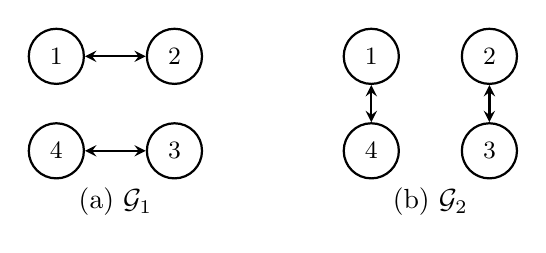
\begin{tikzpicture}[
			agent/.style={
				circle,
				draw,
				thick,
				minimum size=7mm,
				inner sep=0pt,
				font=\small
			},
			edge/.style={
				thick,
				<->,
				>=stealth
			}
			]
			\begin{scope}
				\node[agent] (g11) at (0,1.2) {1};
				\node[agent] (g12) at (1.5,1.2) {2};
				\node[agent] (g14) at (0,0) {4};
				\node[agent] (g13) at (1.5,0) {3};
				\draw[edge] (g11) -- (g12);
				\draw[edge] (g14) -- (g13);
				\node at (0.75,-0.65) {(a) $\mathcal G_1$};
			\end{scope}
			
			\begin{scope}[xshift=4.0cm]
				\node[agent] (g21) at (0,1.2) {1};
				\node[agent] (g22) at (1.5,1.2) {2};
				\node[agent] (g24) at (0,0) {4};
				\node[agent] (g23) at (1.5,0) {3};
				\draw[edge] (g21) -- (g24);
				\draw[edge] (g22) -- (g23);
				\node at (0.75,-0.65) {(b) $\mathcal G_2$};
			\end{scope}
		\end{tikzpicture}
		\caption{Candidate communication topologies.}
		\label{fig:topologies}
	\end{figure}
	
	The corresponding reduced matrices satisfy
	$
	\sigma(\bar A_1)
	=
	\sigma(\bar A_2)
	=
	\{-2,-2,0\},
	$
	and hence neither subsystem is Hurwitz. For
	$
	\lambda=[0.5,0.5]^\top,
	$
	the convex combination satisfies
	$
	\sigma(\bar A_\lambda)
	=
	\{-2,-1,-1\},
	$
	which verifies Lemma~\ref{lem:average}.
	
	Choose
	$
	\Pi
	=
	\begin{bmatrix}
		-0.27&0.27\\
		0.27&-0.27
	\end{bmatrix},
	$
	$
	C=I_3.
	$
	Theorem~\ref{thm:feasibility} gives
	$
	T_{\rm ub}=0.1647~{\rm s}.
	$
	Accordingly, the prescribed dwell time is selected as
	$
	T=0.1~{\rm s}<T_{\rm ub},
	$
	for which the Lyapunov-Metzler inequalities are feasible.
	
	For
	$
	x(0)=[5,-3,4,2]^\top,
	$
	$
	\sigma(0)=1,
	$
	the simulation results are shown in
	Figs.~\ref{fig:state} and~\ref{fig:switch}.
	
	\begin{figure}[H]
		\centering
		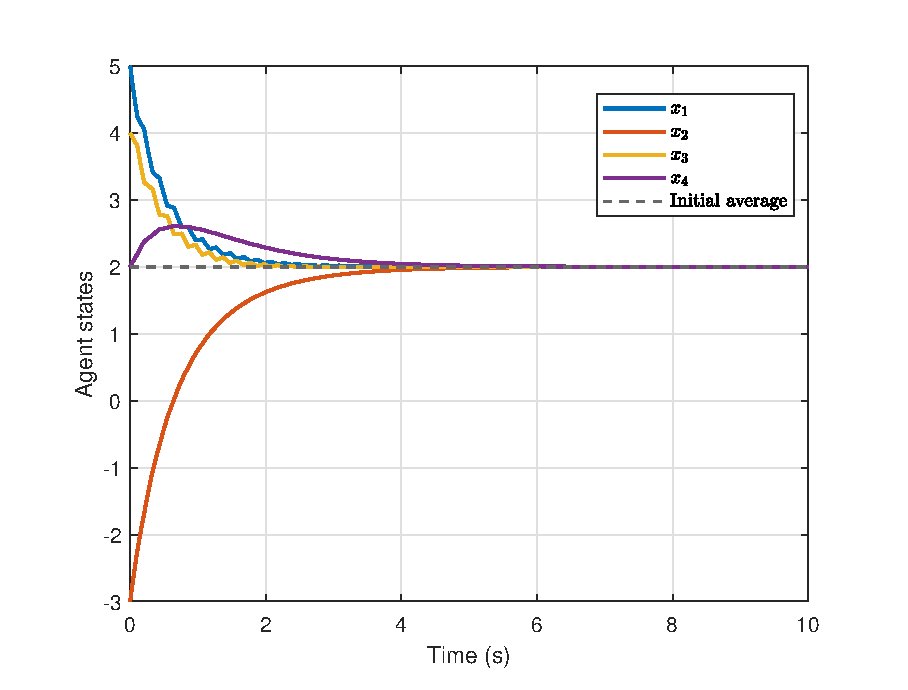
\includegraphics[width=0.8\linewidth,height=4.5cm]{fig_state.eps}
		\caption{Agent state trajectories under the proposed switching law.}
		\label{fig:state}
	\end{figure}
	
	\begin{figure}[H]
		\centering
		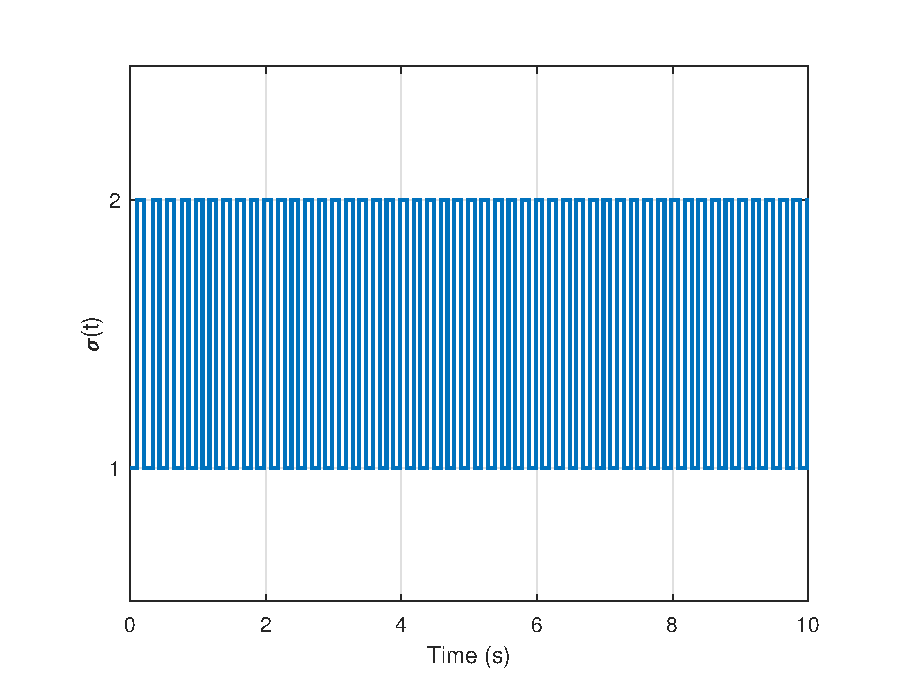
\includegraphics[width=0.8\linewidth,height=4.5cm]{fig_switching.eps}
		\caption{State-dependent switching signal.}
		\label{fig:switch}
	\end{figure}
	
	The agent states converge to the common value $2$, while every
	switching interval is no less than the prescribed dwell time
	$T=0.1~{\rm s}$. Therefore, consensus is achieved although neither
	candidate topology can independently guarantee global consensus.
	
	\section{Conclusion}
	
	This paper studied the consensus problem for multi-agent systems under switching directed topologies. A consensus-orthogonal decomposition was used to transform the original problem into stabilization of a reduced-order switched disagreement system. A state-dependent switching law with a prescribed minimum dwell time was developed based on Lyapunov-Metzler inequalities. Under the joint strong connectivity of the candidate topology
	family, a Hurwitz convex combination of the reduced subsystem
	matrices was obtained and used to construct a Metzler matrix. The feasibility of the Lyapunov-Metzler inequalities were established and an explicit sufficient upper bound on the dwell time was derived. Numerical results demonstrated that consensus can be achieved even when none of the individual subsystem matrices is Hurwitz.
	
	\begin{thebibliography}{00}
		
		\bibitem{olfati2007}
		R.~Olfati-Saber, J.~A. Fax, and R.~M. Murray,
		``Consensus and cooperation in networked multi-agent systems,''
		\emph{Proceedings of the IEEE},
		vol.~95, no.~1, pp.~215--233, 2007.

\bibitem{wen2021book}
		G.~Wen, W.~Yu, Y.~Lv, and P.~Wang,
		\emph{Cooperative Control of Complex Network Systems with
			Dynamic Topologies}.
		Boca Raton, FL, USA: CRC Press, 2021.		
		\bibitem{fu2019constraints}
		J.~Fu, G.~Wen, W.~Yu, T.~Huang, and X.~Yu,
		``Consensus of second-order multiagent systems with both velocity
		and input constraints,''
		\emph{IEEE Transactions on Industrial Electronics},
		vol.~66, no.~10, pp.~7946--7955, 2019.
		
		\bibitem{zhao2015finite}
		Y.~Zhao, Z.~Duan, and G.~Wen,
		``Finite-time consensus for second-order multi-agent systems with
		saturated control protocols,''
		\emph{IET Control Theory \& Applications},
		vol.~9, no.~3, pp.~312--319, 2015.
		
		\bibitem{zhao2019tracking}
		D. Zhao, Y. Lv, X. Yu, G. Wen, and G. Chen, ``Resilient consensus of higher order multiagent networks: An attack isolation-based approach"
		\emph{IEEE Transactions on Automatic Control},
		vol.~67, no.~2, pp.~1001--1007, 2022.
		
		
		
		\bibitem{olfati2004}
		R.~Olfati-Saber and R.~M. Murray,
		``Consensus problems in networks of agents with switching topology
		and time-delays,''
		\emph{IEEE Transactions on Automatic Control},
		vol.~49, no.~9, pp.~1520--1533, 2004.

       
		
		\bibitem{jadbabaie2003}
		A.~Jadbabaie, J.~Lin, and A.~S. Morse,
		``Coordination of groups of mobile autonomous agents using nearest
		neighbor rules,''
		\emph{IEEE Transactions on Automatic Control},
		vol.~48, no.~6, pp.~988--1001, 2003.
		
		\bibitem{ren2005}
		W.~Ren and R.~W. Beard,
		``Consensus seeking in multiagent systems under dynamically
		changing interaction topologies,''
		\emph{IEEE Transactions on Automatic Control},
		vol.~50, no.~5, pp.~655--661, 2005.
		
		\bibitem{wen2014tracking}
		G.~Wen, Z.~Duan, G.~Chen, and W.~Yu,
		``Consensus tracking of multi-agent systems with Lipschitz-type
		node dynamics and switching topologies,''
		\emph{IEEE Transactions on Circuits and Systems I:
			Regular Papers},
		vol.~61, no.~2, pp.~499--511, 2014.
		
		\bibitem{wen2019multiple}
		G.~Wen and W.~X. Zheng,
		``On constructing multiple Lyapunov functions for tracking
		control of multiple agents with switching topologies,''
		\emph{IEEE Transactions on Automatic Control},
		vol.~64, no.~9, pp.~3796--3803, 2019.
		
		
		
		\bibitem{cheng2019}
		B.~Cheng, X.~Wang, and Z.~Li,
		``Event-triggered consensus of homogeneous and heterogeneous
		multiagent systems with jointly connected switching topologies,''
		\emph{IEEE Transactions on Cybernetics},
		vol.~49, no.~12, pp.~4421--4430, 2019.
		
		\bibitem{li2023}
		Y.~Li, F.~Wang, M.~Sader, Z.~Liu, and Z.~Chen,
		``Fault-tolerant consensus of leader--following multi-agent systems
		with jointly connected topologies,''
		\emph{Transactions of the Institute of Measurement and Control},
		vol.~45, no.~9, pp.~1747--1754, 2023.
		
		\bibitem{wang2024protocol}
		J.~Wang, L.~Zhou, D.~Zhang, J.~Liu, and Y.~Zheng,
		``Protocol selection for second-order consensus against
		disturbance,''
		\emph{Automatica},
		vol.~161, Art.~no.~111497, 2024.
		
		\bibitem{liberzon2003}
		D.~Liberzon,
		\emph{Switching in Systems and Control}.
		Boston, MA, USA: Birkh\"auser, 2003.
		
		\bibitem{geromel2006}
		J.~C. Geromel and P.~Colaneri,
		``Stability and stabilization of continuous-time switched linear
		systems,''
		\emph{SIAM Journal on Control and Optimization},
		vol.~45, no.~5, pp.~1915--1930, 2006.
		
		\bibitem{zhai2001}
		G.~Zhai, B.~Hu, K.~Yasuda, and A.~N. Michel,
		``Stability analysis of switched systems with stable and unstable
		subsystems: An average dwell time approach,''
		\emph{International Journal of Systems Science},
		vol.~32, no.~8, pp.~1055--1061, 2001.
		
		\bibitem{jin2023}
		C.-L.~Jin, Q.-G.~Wang, R.~Wang, and D.~Wu,
		``Stabilization of switched systems with unstable modes via
		mode-partition-dependent ADT,''
		\emph{Journal of the Franklin Institute},
		vol.~360, no.~2, pp.~1308--1326, 2023.
		
		\bibitem{yin2023}
		H.~Yin, B.~Jayawardhana, and S.~Trenn,
		``Stability of switched systems with multiple equilibria:
		A mixed stable--unstable subsystem case,''
		\emph{Systems \& Control Letters},
		vol.~180, Art.~no.~105622, 2023.
		
		\bibitem{russo2025}
		A.~Russo, G.~P. Incremona, and P.~Colaneri,
		``Stabilization of switched affine systems with dwell-time
		constraint,''
		\emph{IEEE Transactions on Automatic Control},
		vol.~71, no.~5, pp.~3030--3043, 2026.
		
		\bibitem{hiriart2012}
		J.-B. Hiriart-Urruty and J.~Malick,
		``A fresh variational-analysis look at the positive semidefinite
		matrices world,''
		\emph{Journal of Optimization Theory and Applications},
		vol.~153, no.~3, pp.~551--577, 2012.
		
		\bibitem{nagumo1942}
		M.~Nagumo,
		``\"Uber die Lage der Integralkurven gew\"ohnlicher
		Differentialgleichungen,''
		\emph{Proceedings of the Physico-Mathematical Society of Japan,
			3rd Series},
		vol.~24, pp.~551--559, 1942.
		
	\end{thebibliography}
	
\end{document}
